%%%%%%%%%%%%%%%%%%%%%%%%%%%%%%%%%%%%%%%%%
% Stylish Article
% LaTeX Template
% Version 2.1 (1/10/15)
%
% This template has been downloaded from:
% http://www.LaTeXTemplates.com
%
% Original author:
% Mathias Legrand (legrand.mathias@gmail.com)
% With extensive modifications by:
% Vel (vel@latextemplates.com)
%
% License:
% CC BY-NC-SA 3.0 (http://creativecommons.org/licenses/by-nc-sa/3.0/)
%
%%%%%%%%%%%%%%%%%%%%%%%%%%%%%%%%%%%%%%%%%

%----------------------------------------------------------------------------------------
%  PACKAGES AND OTHER DOCUMENT CONFIGURATIONS
%----------------------------------------------------------------------------------------
\documentclass[10pt]{SelfArx} % Document font size and equations flushed left

%fleqn,
\usepackage[T1]{fontenc}
\usepackage{newtxmath,newtxtext}

\usepackage{textcomp}
\usepackage{gensymb}
\usepackage{multirow}

\usepackage{amsmath, amsfonts}

\usepackage{titlesec}
\usepackage{subfigure}
%\titlespacing*{\section}{-0.5pt}{0.5\baselineskip}{\baselineskip}
%\usepackage[english]{babel} % Specify a different language here - english by default

%----------------------------------------------------------------------------------------
%  COLUMNS
%----------------------------------------------------------------------------------------

\setlength{\columnsep}{0.55cm} % Distance between the two columns of text
\setlength{\fboxrule}{0.75pt} % Width of the border around the abstract

%----------------------------------------------------------------------------------------
%  COLORS
%----------------------------------------------------------------------------------------

\definecolor{color1}{RGB}{0,0,90} % Color of the article title and sections
\definecolor{color2}{RGB}{0,20,20} % Color of the boxes behind the abstract and headings

%  HYPERLINKS
%----------------------------------------------------------------------------------------

\usepackage{hyperref} % Required for hyperlinks
\hypersetup{hidelinks,colorlinks,breaklinks=true,urlcolor=color2,citecolor=color1,linkcolor=color1,bookmarksopen=false,pdftitle={Title},pdfauthor={Author}}

%----------------------------------------------------------------------------------------
%  ARTICLE INFORMATION
%----------------------------------------------------------------------------------------

\JournalInfo{ORIE 4741: Learning With Big Messy Data} % Journal information
\Archive{December 2, 2017} % Additional notes (e.g. copyright, DOI, review/research article)

\PaperTitle{Predicting Arrests in the Murder Capital of America} % Article title


\Authors{Bridget Cheng (bjc267), Celine Brass (cjb327), Reuben Rappaport (rbr76)} % Authors

\Keywords{} % Keywords - if you don't want any simply remove all the text between the curly brackets
\newcommand{\keywordname}{Keywords} % Defines the keywords heading name

%----------------------------------------------------------------------------------------
%  ABSTRACT
%----------------------------------------------------------------------------------------

\Abstract{Chicago, a city with a homicide rate so bad it's anecdotally known as the murder capital of America, has a chronically high crime. And yet, of the countless crimes reported, only a few will eventually lead to an arrest. When the crime rate is so high to begin with, systemic analysis of police efficacy is called for. In this report we set out to analyze which types of crimes lead to an arrest and more importantly, which don't. Based on this analysis we create a set of recommendations for reallocating police resources.}

%----------------------------------------------------------------------------------------

\newlength\tindent
\setlength{\tindent}{\parindent}
\setlength{\parindent}{0pt}
\renewcommand{\indent}{\hspace*{\tindent}}

\begin{document}



\flushbottom % Makes all text pages the same height

\noindent \maketitle % Print the title and abstract box


% \tableofcontents % Print the contents section

\thispagestyle{empty} % Removes page numbering from the first page

%----------------------------------------------------------------------------------------
%  ARTICLE CONTENTS
%----------------------------------------------------------------------------------------

\section{Introduction} % The \section*{} command stops section numbering
We set out to predict the probability of an arrest being made for a crime occurring at a given time and place in the city of Chicago. Chicago, with its famously high crime rate, and heavy municipal investment in making its data available online is a natural target for analysis of police effectiveness. We used the CLEAR dataset which lists all reported crimes from 2001 until the present day (with the exception of murder) to build our model.

This sort of analysis can lead to insights into deficiencies in policing - perhaps certain areas of the city are systematically under-policed or certain types of crime are systematically under-investigated. Analyzing the nature and features of crimes committed in the past to identify these biases will allow us to improve the dispatchment of our police force and procedures for handling specific types of crime in the future.

\section{Exploratory Data Analysis}

    \subsection{CLEAR Dataset}
    The Chicago Police Department maintains a CLEAR (Citizen Law Enforcement Analysis and Reporting) database of committed crimes from 2001 to the present day, detailing characteristics about the incident including the type, location, time, and descriptions of the police force tasked with resolving the incident. This database is consistently maintained and updated daily to reflect the most recent history of crimes. The CLEAR dataset contains over 6 million rows and 22 columns, providing us with a large amount of data for train and test. The dataset contains primarily quantitative data; however, more detailed descriptions of the location and type of crime are provided qualitatively. Since it was complete, well formatted, and easily accessible we elected to use this dataset as the basis of our analsysis.

    \subsection{Features}
    Each entry in the CLEAR dataset contains the following features:

    \begin{itemize}
        \item \textbf{Arrest:} Whether or not an arrest was made. This is the output of our logistic regression model.
        \item \textbf{ID:} A unique identifier for each record
        \item \textbf{Case Number:} The Chicago Police Department Records Division Number
        \item \textbf{Date:} The date the incident supposedly occurred
        \item \textbf{Block:} A partially redacted address where the incident occurred, placing it on the same block as the incident
        \item \textbf{IUCR:} Illinois Uniform Crime Reporting Code. This encodes both the primary type of the incident and a secondary description
        \item \textbf{Primary Type:} The primary description encoded by the IUCR code
        \item \textbf{Description:} The secondary description encoded by the IUCR code
        \item \textbf{Location Description:} A description of the location where the incident occurred. Ex : STREET, APARTMENT, etc
        \item \textbf{Domestic:} A binary variable indicating whether or not the incident was domestic-related
        \item \textbf{Beat:} The beat where the incident occurred. A beat is an area of Chicago assigned to a single patrolling police car
        \item \textbf{District:} The police district where the incident occurred
        \item \textbf{Ward:} The city council district where the incident occurred
        \item \textbf{Community Area:} The Chicago community area where the incident occurred
        \item \textbf{FBI Code:} The crime classification as outlined by the FBI’s National Incident-Based Reporting System
        \item \textbf{X Coordinate:} The x coordinate of the location (partially redacted) of the incident
        \item \textbf{Y Coordinate:} The y coordinate of the location (partially redacted) of the incident
        \item \textbf{Year:} The year the incident occurred
        \item \textbf{Updated on:} The date and time the record was last updated in the database
        \item \textbf{Latitude:} The latitude of the partially redacted location of the incident
        \item \textbf{Longitude:} The longitude of the partially redacted location of the incident
        \item \textbf{Location:} The partially redacted location of the incident in a format suitable for mapping
    \end{itemize}

    Looking at these features, we noticed that there was a great deal of redundancy. The Block, Beat, District, Ward, Community Area, X Coordinate, Y Coordinate, Latitude, Longitude, and Location features all provided some encoding of the crime location. Similarly, the IUCR, Primary Type, Description, and FBI Code, all provided an encoding of the crime's type. To get a better sense for which features were actually important we moved on to making data visualizations.

    \subsection{Data Visualizations}
    Before attempting to choose a model for this dataset, we generated several initial histograms and plots. These helped us to better understand how the data was distributed and which features were worth focusing on

    \begin{figure}[h]
      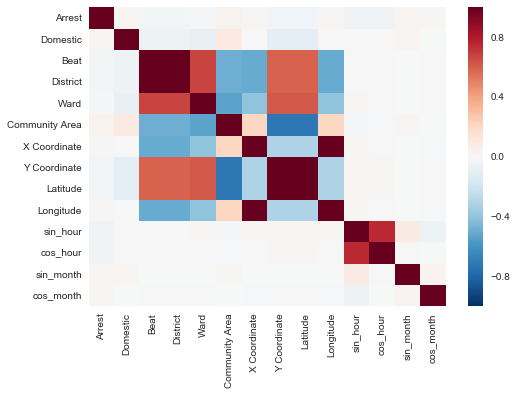
\includegraphics[width=\linewidth]{FinalVisualizations/correlation.png}
      \caption{Heatmap of the correlation between features}
      \label{fig:corr}
    \end{figure}

    Consider Figure~\ref{fig:corr}. This heatmap depicts the correlations between each of the features present in the original dataset. As you can see, there is a high correlation between the \textbf{Beat, District, Ward, Community Area, X Coordinate, Y Coordinate, Latitude,} and \textbf{Longitude}. This makes sense considering that all of these variables describe the crime's location. However since many models rely on independent features, we decided it would be best to pick a single encoding to keep and drop the others.

    \begin{figure}[h]
      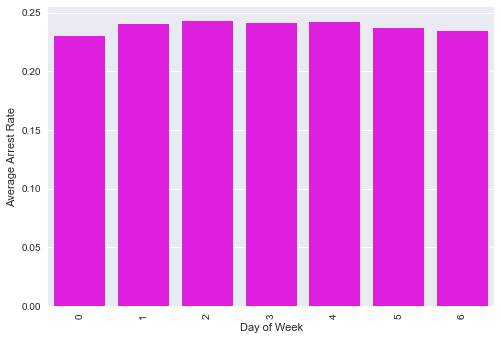
\includegraphics[width=\linewidth]{FinalVisualizations/dayofweek.png}
      \caption{Bar plot showing arrest rate by the day of the week}
      \label{fig:weekday}
    \end{figure}

    \begin{figure}[h]
      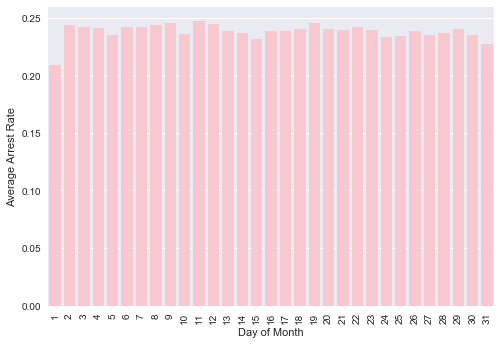
\includegraphics[width=\linewidth]{FinalVisualizations/dayofmonth.png}
      \caption{Bar plot showing arrest rate by the day of the month}
      \label{fig:monthday}
    \end{figure}

    Consider Figure~\ref{fig:weekday} and Figure~\ref{fig:monthday}. These figures depict respectively the arrest rate by day of the week and the arrest rate by day of the month. To our surprise, there did not seem to be a significant correlation between either of these variables and the arrest rate. Because of this we elected to drop them from our final model.

    \begin{figure}[h]
      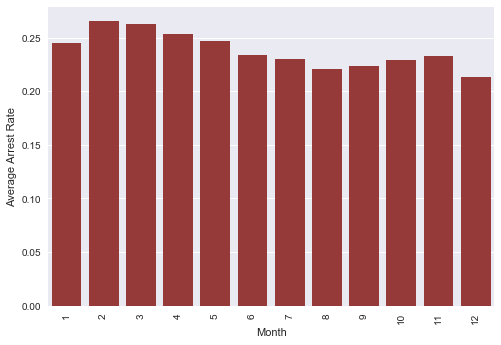
\includegraphics[width=\linewidth]{FinalVisualizations/month.png}
      \caption{Bar plot showing arrest rate by month}
      \label{fig:month}
    \end{figure}

    \begin{figure}[h]
      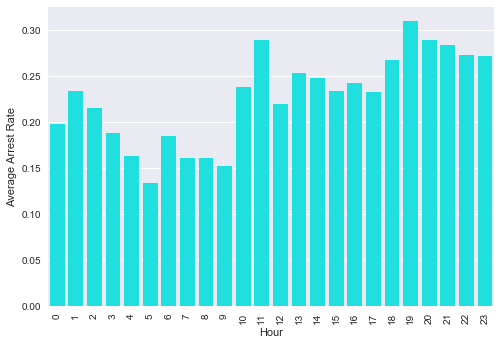
\includegraphics[width=\linewidth]{FinalVisualizations/hour.png}
      \caption{Bar plot showing arrest rate by hour of the day}
      \label{fig:hour}
    \end{figure}

    Consider Figure~\ref{fig:hour} and Figure~\ref{fig:month} which show the arrest
    rate by hour of the day and by month of the year. There's a very noticeable correlation between hour and arrest rate, with arrests rising in the evening before dropping in the early morning. The correlation with month is less noticeable but is still prominent enough for us to consider it in our model.

    \begin{figure}[h]
      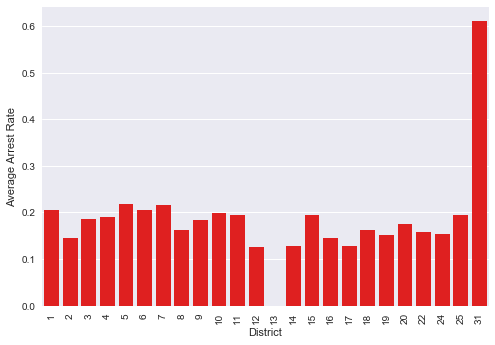
\includegraphics[width=\linewidth]{FinalVisualizations/district.png}
      \caption{Bar plot showing arrest rate by district}
      \label{fig:district}
    \end{figure}

    \begin{figure}[h]
      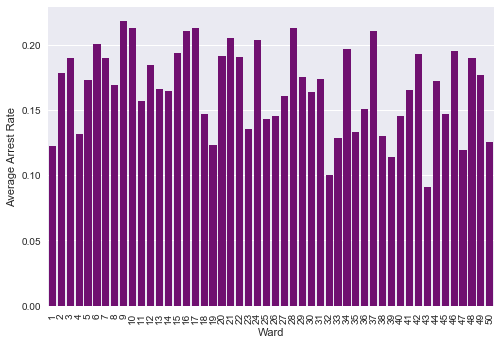
\includegraphics[width=\linewidth]{FinalVisualizations/ward.png}
      \caption{Bar plot showing arrest rate by ward}
      \label{fig:ward}
    \end{figure}

    Figure~\ref{fig:ward} and Figure~\ref{fig:district} show the arrest rate by
    ward and by district respectively. Both of these location groupings show
    a variation in arrest rate. However district has two bizarre outliers -
    district 13 which has no arrests at all, and district 31 which has an arrest
    rate near 1.0. We suspect that Chicago is similar to the Hunger Games and district
    13 may not actually exist. Because of this we chose to include ward in our
    final model rather than district.

    \begin{figure}[h]
      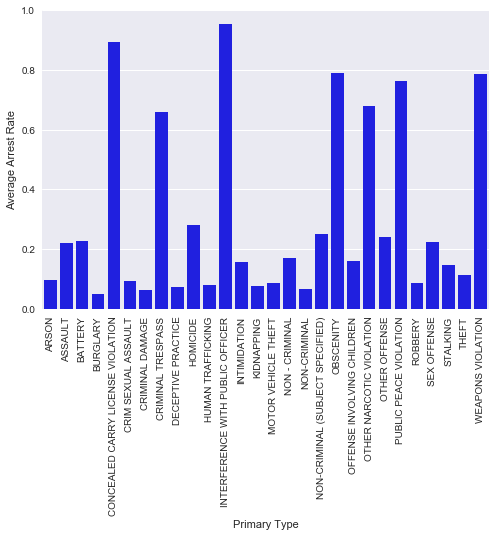
\includegraphics[width=\linewidth]{FinalVisualizations/primarytypes.png}
      \caption{Bar plot showing arrest rate by crime type}
      \label{fig:primarytype}
    \end{figure}

    Figure~\ref{fig:primarytype} shows the arrest rate by type of crime. As you
    can see, there is an extremely wide spread, suggesting that this feature
    may have major effects. Based on this we decided to keep crime type in the
    model.

    \subsection{Data Cleaning}
    The original dataset required significant manipulation before it was ready to be used.

        \subsubsection{Discarded Features}
        Using the initial data visualizations, we were able to identify which features we believed would be informative to our model. Of the original 22 features present, we chose to completely discard the following features from the dataset:
        \begin{itemize}
            \item \textbf{ID, Case Number, Updated On:} These features provide no descriptive information about the crime.
            \item \textbf{IUCR:} This feature is a numeric encoding of both the Primary Type and Description features, we decided to remove the single IUCR feature in favor of the two distinct categorical features
            \item \textbf{Block, Beat, District, Community Area, X Coordinate, Y Coordinate, Latitude, Longitude, Location:} These features provide location description in varying granularities. Several of these features were dropped because of their incredibly large unique value count--it is very unlikely that a model would be able to suitably use these features for differentiation. The remainder of these features were dropped because of their uniform arrest rates across values. From our generated visualizations, it was clear that the location-based feature that had most variation across arrest rates was Ward, hence we decided use this feature as the only location encoding in our dataset.
        \end{itemize}

        \subsubsection{Time and Date Segmentation}
        To address the Date feature, we first segmented the string value into two new features, Hour and Month. We chose to disregard the Day of Month and Day of Week features initially used in the visualizations, as we saw the distribution of arrests was almost uniform over days of the month and days of the week. Furthermore, because representing hour and month as integers does not represent the cyclic nature of these values, we cleverly applied a sine and cosine transformation function to the values, so that the closeness of values like 0 and 23 in the hours of a day is captured despite a large numerical difference. This introduced four new features, Sin Hour, Cos Hour, Sin Month, and Cos Month. We removed the original Date feature as a final step.

        \subsubsection{Categorical to Quantitative Data}
        Categorical features need processing to be represented in the dataset as quantitative binary values. To do this, we utilized one-hot encodings for each value that the categorical feature took on. This process, known as creating dummy variables, indicates the presence or absence of a categorical effect. For example, for each of the possible Primary Type values, "Robbery", "Prostitution", "Ritualism", etc., a new feature "Primary\_Type\_Robbery", "Primary\_Type\_Prostitution", "Primary\_Type\_Ritualism", etc. was introduced with a value of 0 or 1 depending on the value of the original Primary Type feature.

        The boolean true and false values of the Arrest and Domestic features were simply transformed to be binary 0 and 1 values.

        \subsubsection{Limiting the Data}
        To limit the size of our data, we decided to use only reports that have taken place in the last 5 years--this left only crimes reported between the years of 2013-present day. Furthermore, we noticed from our visualizations that crimes of particular Primary Type values had arrest rates of nearly 1--we immediately attributed this to the fact that certain crimes would only be reported if an arrest were definitely going to be made, for example, liquor law violations or public indecency violations. We manually inspected the various Primary Type values, and ultimately chose to remove crimes with Primary Type of Gambling, Liquor Law Violation, Prostitution, Narcotics, and Public Indecency. Rows for which data were missing were also dropped. The final dataset contained over 900,000 rows.

\section{Model Selection}
We used three different classification techniques on our dataset: logistic regression, decision trees, and a Naive Bayes classifier. For all of the models, we used an 80\% training set and a 20\% test set.

    \subsection{Logistic Regression}
    Many predictive models apply an absolute prediction to each sample, however it is not the case that a crime of a given type committed at a given time and place will deterministically result in an arrest or not. It is perfectly possible for nearly identical crimes to have different outcomes. Based on this structure we determined that a relevant approach would be to predict the probability that a crime with certain features would lead to an arrest. A natural model to perform this translation between binary outcomes and statistical probabilities is logistic regression. We decided to train two separates models, one using an $L1$ regularizer and another using an $L2$ regularizer. Because the number of features increased dramatically with the use of dummy variables, we believed that an $L1$ regularizer could help to encourage sparsity and therefore interpretability.

    \subsection{Gaussian Naive Bayes}
    A popular alternative to logistic regression for classification is a Naive Bayes classifier. In particular, we used a Gaussian Naive Bayes classifier. Given the features $X$ and outcome $y$, a Naive Bayes algorithm estimates the joint probability from the training data using the well-known Bayes Theorem.

        \begin{equation}
         P(c_j | x)= \dfrac{P(x|c_j)P(c_j)}{P(x)}
        \end{equation}

    In Naive Bayes, feature weights are fit independently; i.e. they depend on how much that feature correlates with the outcome. This is in contrast to logistic regression, which determines all the weights as a function of the loss. It is important to note that the Naive Bayes classifier assumes that all features are conditionally independent, hence the "naivete" of the method. We decided to use this approach as a comparison to the logistic regression.

    \subsection{Decision Tree}
    Another approach we used was fitting a decision tree. A decision tree attempts to create axis-aligned linear decision boundaries. Decisions have high interpretability and can account for interations between features. Decision trees tend to have lower performance rates--something that they tradeoff for interpretability; however, because a large part of our analysis is meant to understand the Chicago police force, we felt that this approach could provide some valuable insight.

\section{Results}
    \subsection{Logistic Regression}
    The L1 and L2 regularizers had similar classification reports, but we believe L1 to be slightly more interpretable due to the sparsity of its solution--only 177 of the 466 were non-zero.

    The L1 regularized logistic regression performed with an average accuracy of 87.7\% on our test set. The following confusion matrix represents the distribution of false positives, false negatives, true positives, and true negatives.

    \begin{tabular}{l|l|c|c|c}
    \multicolumn{2}{c}{}&\multicolumn{2}{c}{Predicted Outcome}&\\
    \cline{3-4}
    \multicolumn{2}{c|}{}&No Arrest&Arrest&\multicolumn{1}{c}{Total}\\
    \cline{2-4}
    \multirow{2}{*}{True Outcome}& No Arrest & 145854 & 3278 & 149132\\
    \cline{2-4}
    & Arrest & 18684  & 13142 & 31826\\
    \cline{2-4}
    \multicolumn{1}{c}{} & \multicolumn{1}{c}{Total} & \multicolumn{1}{c}{164538} & \multicolumn{    1}{c}{16420} &
    \multicolumn{1}{c}{180958}\\
    \end{tabular}

    The following table provides the precision, recall, and f1-score of the model.

    \begin{center}
        \begin{tabular}{|c | c | c | c| c|}
        \hline
        & Precision & Recall & F1-Score & Support \\ [0.5ex]
        \hline\hline
        0 & 0.89 & 0.98 & 0.93 & 149132 \\
        \hline
        1 & 0.80 & 0.41 & 0.54 & 31826 \\
        \hline
        avg / total & 0.87 & 0.88 & 0.86 & 180958 \\
        \hline
        \hline
        \end{tabular}
    \end{center}

    \subsection{Gaussian Naive Bayes}
    The Gaussian Naive Bayes classifier performed with an average accuracy of 85.1\%

    \begin{tabular}{l|l|c|c|c}
    \multicolumn{2}{c}{}&\multicolumn{2}{c}{Predicted Outcome}&\\
    \cline{3-4}
    \multicolumn{2}{c|}{}&No Arrest&Arrest&\multicolumn{1}{c}{Total}\\
    \cline{2-4}
    \multirow{2}{*}{True Outcome}& No Arrest & 137349 & 11783 & 149132\\
    \cline{2-4}
    & Arrest & 15363 & 16463 & 31826\\
    \cline{2-4}
    \multicolumn{1}{c}{} & \multicolumn{1}{c}{Total} & \multicolumn{1}{c}{152712} & \multicolumn{    1}{c}{28246}&     \multicolumn{1}{c}{180958}\\
    \end{tabular}

    \begin{center}
        \begin{tabular}{|c | c | c | c| c|}
        \hline
        & Precision & Recall & F1-Score & Support \\ [0.5ex]
        \hline\hline
        0 & .90 & 0.92 & 0.91 & 149132 \\
        \hline
        1 & 0.58 & 0.52 & 0.55 & 31826 \\
        \hline
        avg / total & 0.84 & 0.85 & 0.85 & 180958 \\
        \hline
        \hline
        \end{tabular}
    \end{center}

    \subsection{Decision Tree}
    The Gaussian Naive Bayes classifier performed with an average accuracy of 84.8\%

    \begin{tabular}{l|l|c|c|c}
    \multicolumn{2}{c}{}&\multicolumn{2}{c}{Predicted Outcome}&\\
    \cline{3-4}
    \multicolumn{2}{c|}{}&No Arrest&Arrest&\multicolumn{1}{c}{Total}\\
    \cline{2-4}
    \multirow{2}{*}{True Outcome}& No Arrest & 135409 & 13723 & 149132\\
    \cline{2-4}
    & Arrest & 16581 & 15245 & 31826\\
    \cline{2-4}
    \multicolumn{1}{c}{} & \multicolumn{1}{c}{Total} & \multicolumn{1}{c}{151990} & \multicolumn{    1}{c}{28968} &     \multicolumn{1}{c}{180958}\\
    \end{tabular}

    \begin{center}
        \begin{tabular}{|c | c | c | c| c|}
        \hline
        & Precision & Recall & F1-Score & Support \\ [0.5ex]
        \hline\hline
        0 & 0.89 & 0.91 & 0.90 & 149132 \\
        \hline
        1 & 0.53 & 0.48 & 0.50 & 31826 \\
        \hline
        avg / total & 0.83 & 0.83 & 0.83 & 180958 \\
        \hline
        \hline
        \end{tabular}
    \end{center}

    \subsection{Discussion of Results}
    The logistic regression outperformed both the decision tree and the Naive Bayes classifier numerically, though not by a significant amount. The confusion matrices show that all of the models predicted large numbers of true positives and true negatives. Despite attempts to use structured sampling, various classification techniques, and various regularization techniques, we were unable to achieve significant improvement. We ultimately chose to use the logistic regression with an L1 regularizer and simple random sampling. This model won over the similarly performing models because it performed the best on negative outcomes versus positive--something we believe to be more valuable for improving policing.

    For each original feature that was one-hot encoded into multiple new features, we calculated the average absolute value weight of each of those one hot encoded features in the logistic regression solution. This gave us a sense of which of the original features had the greatest effect on whether an arrest was made. The following average absolute weights of the logistic regression for each original feature were calculated:
        \begin{itemize}
            \item Primary Type: .99
            \item Description: .87
            \item Location Type: .34
            \item Ward: .09
        \end{itemize}

    We can see that the Primary Type and Description features seemed to have the most influence on the arrest of a crime. This, although not surprising, is still an insightful result when we account for the fact that the effect of weight of Location and Ward was an order of magnitude smaller.

    \subsection{In Plain English}
    Our final model shows that the greatest indicator for whether or not an arrest will be made is the type of the crime. This is somewhat surprising, as we initially thought that location in the city (Ward, as opposed to the Location Type) would have a more significant effect on the result. Many policing efforts focus on targeting certain areas and locations of a city that are more prone to crime, but it is less often so that we hear about targeted policing efforts for a particular category of crime. Our results suggest that rather than investing extra resources in policing high crime areas, it may be more effective to develop crime-specific policing programs.

\section{Conclusion}

We believe that our results are consistent and accurate enough that they provide valuable insight as to how to improve policing. By using three very different classification techniques, all of which returned similar results, we were able to confirm that there is a predictive relationship between our input and output variables. We support the implementation of our recommendations made in the previous section.

The Chicago Police Department has heavily invested in making all of their crime data available online for public use. By taking advantage of this resource, we have been able to not only analyze the distribution of crime in Chicago, but also train a predictive model, which for a given crime, is able to predict with high accuracy whether an arrest will be made. The techniques we explored in the course guided us in this investigation and allowed us to ultimately work through a complex data analysis problem end-to-end. 

\section{References}
    \begin{itemize}
        \item Chicago Data Portal. (2017). Crimes - 2001 to present.
        https://data.cityofchicago.org/Public-Safety/Crim es-2001-to-present/ijzp-q8t2
    \end{itemize}

\end{document}
